\chapter{Entwicklung eines technischen Objekts}
%TODO Einleitung: Idee
% explizite Bezug auf Ultimaker 2, andere Drucker liefern andere Ergebnisse

Dieses Kapitel handelt vom Entwerfen und Drucken eines technischen Objekts. Als Objekt wird hier exemplarisch ein Aufbewahrungssystem f�r einen Raspberry Pi gekoppelt mit einem \ac{USB}- Hub und einer  externen Festplatte entworfen. Dieses System soll m�glichst kompakt sein und als ein Block transportierbar sein.

Diese Arbeit bezieht sich h�ufig auf den ultimaker 2, der im vorhergehenden Kapitel \ref{chapter:techGr:ultimaker2} vorgestellt wird. In der Arbeit mit einem anderen Drucker k�nnen sich Vorgehensweise und Ergebnis deutlich unterscheiden.

Zuerst wird die Analyse der bestehenden Verwahrung beschrieben. Anschlie�end folgt eine Beschreibung des umzusetzenden Konzepts. Folgend wird ein Entwurf des Systems mit einem \ac{CAD}-Programm  und der Druck des Objekts beschrieben. Der darauffolgende Abschnitt besch�ftigt sich mit w�hrend dem Druck aufgetretenen Fehlern. Zuletzt folgt ein Fazit �ber die Eignung des ultimaker 2 zum Drucken von technischen Objekten.


%TODO Ist-Analyse
\newpage
\section{Ist-Analyse}
	\piccaption{Urspr�ngliches Stapelsystem}
	\parpic{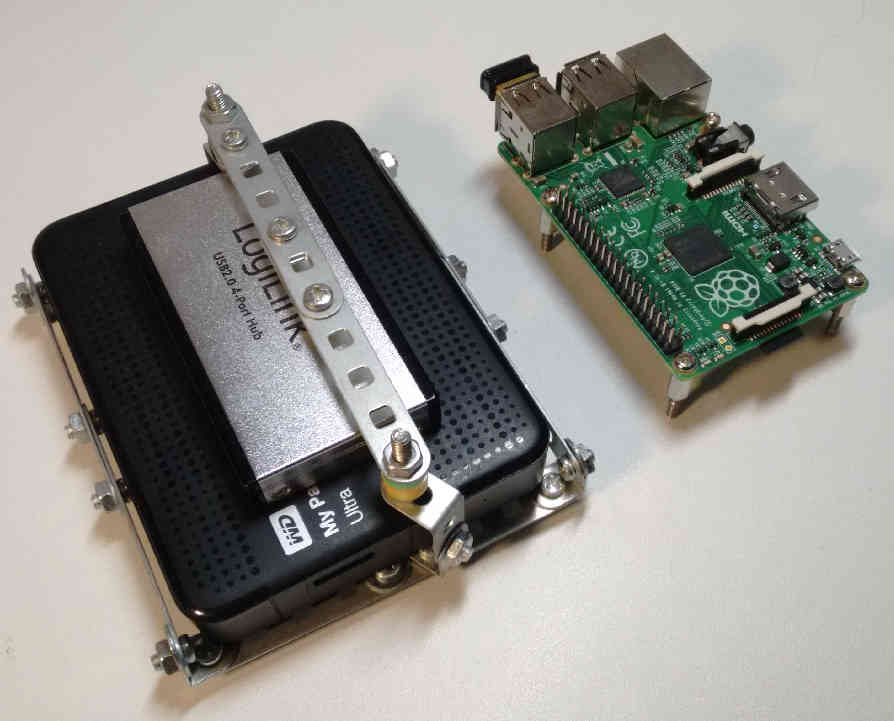
\includegraphics[width=.5\textwidth]{images/techObj/urspruenglicheHalterung02.jpg}}
	
	\picskip{0}
	
%TODO 
\section{Konzept: Modulare Boxen}

\section{Entwurf}
%Erw�hnen, dass Solid Edge verwendet

\section{Druck des Objekts}
% Wie w�re es ideal gewesen?, fertiges Objekt 
% Welche Parameter? --> spezifisch beim technischen Objekt
% Verlinkung zu Fehlern

\section{Aufgetretene Fehler}
% Bilder
% Fehleranalyse, [Ma�nahmen --> technische Grundlagen]

\section{Fazit: Eignung f�r technische Objekte}
% bezogen auf Ultimaker
Wie bereits eingangs erw�hnt, wurde f�r diese Studienarbeit der Ulitmaker 2 verwendet. Deshalb kann in diesem Fazit auch nur betrachtet werden, inwiefern sich dieser Drucker eignet, um technische Objekte zu erstellen.\\

\subsection{Material}
Als Plastik wurde PLA verwendet. Bei den Drucken fiel auf, dass die Materialeigenschaften, abh�ngig von der verwendeten Farbe, teilweise deutlich unterschiedlich waren. Am besten gelangen die Drucke mit rotem Filament. Schwarzes Filament dagegen war sehr spr�de. Bei durchsichtigem Filament hielten die verschiedenen Linien nicht so stark zusammen wie beispielsweise bei rotem, was insbesondere bei konzentrischen Mustern zu einer Instabilit�t f�hrte.\\
F�r das Aufbewahrungssystem wurde deshalb vor allem rotes Filament genutzt. Allgemein sollte man beim Ultimaker 2 also vor dem Druck eines gr��eren Objekts testen, welche Farbe die besten Eigenschaften aufweist.\\
Die Boxen des Aufbewahrungssystems wurden mit Wand- und Bodendicken von 3mm angefertigt, die Bodenplatte des Systems mit einer noch h�heren Bodendicke. Dadurch war das System stabil genug, um hochgehalten zu werden. 


\subsection{Liniendicke} 
Zu dem Zeitpunkt, zu dem das technische Objekt gedruckt wurde, stand nur eine Nozzle der Gr��e 0.4mm zur Verf�gung. Dadurch ist die minimale Breite einer Linie festgelegt. F�r das Aufbewahrungssystems mussten keine Strukturen, die feiner als 0.4mm sind, gedruckt werden. F�r dieses Objekt war die Genauigkeit also hoch genug. \\
M�ssen dagegen Objekte mit feineren Strukturen gedruckt werden, kann es sein, dass der Ultimaker 2 nicht die n�tige Genauigkeit besitzt.
Eine Abhilfe stellt der Olsson Block dar. Dabei handelt es sich um ein Upgrade des Heizblocks, das f�r den Ulitmaker 2 erworben werden kann. Dieses Upgrade erm�glicht es, die Druckd�sen relativ einfach auszutauschen. Im Upgrade sind vier verschieden gro�e D�sen enthalten, die zwischen 0.25 und 0.8mm dick sind. 
Trotz allem bleibt die minimale Dicke einer Linie also auf 0.25mm begrenzt.

% TODO: m�gliche Erkl�rung, warum H�henunterschied ()?)
\subsection{H�he}
Um zu testen, wie pr�zise der Ultimaker 2 die gew�nschte H�he von Objekten drucken kann, wurde ein einfaches Testobjekt gedruckt. Dieses Testobjekt war ein Quader, dessen Ma�e 10x10x1mm waren. Nach dem Druck wurde die tats�chliche H�he des gedruckten Objekts mit einer Schieblehre gemessen. Das gedruckte Objekt war jedoch nur 0.8mm hoch. \\
F�r das Aufbewahrungssystem war diese Genauigkeit ausreichend. Da technische Objekte jedoch mit minimalen Abweichungen angefertigt werden sollten, ist diese Abweichung an sich zu deutlich. Sie zeigt, dass der Ultimaker 2 nicht die notwendige Pr�zision liefern kann, die f�r technische Objekte oft notwendig ist.
